\documentclass{article}
\usepackage{amsmath}
\usepackage{amssymb}
\usepackage{amsthm}
\usepackage[noend]{algpseudocode} 
\usepackage{algorithm}
\usepackage{subfigure}
\usepackage{enumitem}
\usepackage{pgf,tikz}
\usepackage{pgfplots}

\pgfplotsset{
    compat=1.15,
    %every axis legend/.append style={at={(0.5,-0.13)},anchor=north,legend cell align=left},
    legend pos=north west,
    legend style={draw=none,
              text width=0.9in,           %% adjust
              %minimum height=0.5in,     %% adjust
              %anchor=center,
              %cells={anchor=west},
            },
    %axis lines=left,
}
\usetikzlibrary{calc}
\usepackage{graphicx}
\newcommand{\acm}[3]{\{#1\}\rightarrow#3}
\newcommand{\ac}[3]{$\{#1\}\rightarrow#3$}
\newcommand{\omesi}{^\omega_\varsigma}
\usepackage{url}
% Macros relatives à la traduction de PH avec arcs neutralisants vers PH à k-priorités fixes

% Macros générales
%\newcommand{\ie}{\textit{i.e.} }
\newcommand{\segm}[2]{\llbracket #1; #2 \rrbracket}
%\newcommand{\f}[1]{\mathsf{#1}}

% Notations générales pour PH
\newcommand{\PH}{\mathcal{PH}}
%\newcommand{\PHs}{\mathcal{S}}
\newcommand{\PHs}{\Sigma}
%\newcommand{\PHp}{\mathcal{P}}
\newcommand{\PHp}{\textcolor{red}{\mathcal{P}}}
%\newcommand{\PHproc}{\mathcal{P}}
\newcommand{\PHproc}{\mathbf{Proc}}
\newcommand{\Proc}{\PHproc}
\newcommand{\PHh}{\mathcal{H}}
\newcommand{\PHa}{\PHh}
%\newcommand{\PHa}{\mathcal{A}}
\newcommand{\PHl}{\mathcal{L}}
\newcommand{\PHn}{\mathcal{N}}

\newcommand{\PHhitter}{\mathsf{hitter}}
\newcommand{\PHtarget}{\mathsf{target}}
\newcommand{\PHbounce}{\mathsf{bounce}}
%\newcommand{\PHsort}{\Sigma}
\newcommand{\PHsort}{\PHs}

%\newcommand{\PHfrappeur}{\mathsf{frappeur}}
%\newcommand{\PHcible}{\mathsf{cible}}
%\newcommand{\PHbond}{\mathsf{bond}}
%\newcommand{\PHsorte}{\mathsf{sorte}}
%\newcommand{\PHbloquant}{\mathsf{bloquante}}
%\newcommand{\PHbloque}{\mathsf{bloquee}}

%\newcommand{\PHfrappeR}{\textcolor{red}{\rightarrow}}
%\newcommand{\PHmonte}{\textcolor{red}{\Rsh}}

\newcommand{\PHhitA}{\rightarrow}
\newcommand{\PHhitB}{\Rsh}
%\newcommand{\PHfrappe}[3]{\mbox{$#1\PHhitA#2\PHhitB#3$}}
%\newcommand{\PHfrappebond}[2]{\mbox{$#1\PHhitB#2$}}
\newcommand{\PHhit}[3]{#1\PHhitA#2\PHhitB#3}
\newcommand{\PHfrappe}{\PHhit}
\newcommand{\PHhbounce}[2]{#1\PHhitB#2}
\newcommand{\PHobj}[2]{\mbox{$#1\PHhitB^*\!#2$}}
\newcommand{\PHobjectif}{\PHobj}
\newcommand{\PHconcat}{::}
%\newcommand{\PHneutralise}{\rtimes}
\def\Sce{\mathbf{Sce}}

% Actions plurielles
\newcommand{\PHhitmultsymbol}{\rightarrowtail}
\newcommand{\PHhitmult}[2]{\mbox{$#1 \PHhitmultsymbol #2$}}
\newcommand{\PHfrappemult}{\PHhitmult}
\newcommand{\PHfrappemults}[2]{\PHhitmult{\{#1\}}{\{#2\}}}

\def\PHget#1#2{{#1[#2]}}
%\newcommand{\PHchange}[2]{#1\langle #2 \rangle}
%\newcommand{\PHchange}[2]{(#1 \Lleftarrow #2)}
%\newcommand{\PHarcn}[2]{\mbox{$#1\PHneutralise#2$}}
\newcommand{\PHplay}{\cdot}

\newcommand{\PHstate}[1]{\mbox{$\langle #1 \rangle$}}
\newcommand{\PHetat}{\PHstate}

\def\supp{\mathsf{support}}
\def\first{\mathsf{first}}
\def\last{\mathsf{last}}

\def\DNtrans{\rightarrow_{ADN}}
\def\DNdef{(\mathbb F, \langle f^1, \dots, f^n\rangle)}
\def\DNdep{\mathsf{dep}}
\def\PHPtrans{\rightarrow_{PH}}
\def\get#1#2{#1[{#2}]}
\def\encodeF#1{\mathbf{#1}}
\def\toPH{\encodeF{PH}}
\def\card#1{|#1|}
\def\decode#1{\llbracket#1\rrbracket}
\def\encode#1{\llparenthesis#1\rrparenthesis}
\def\Hits{\PHa}
\def\hit{\PHhit}
\def\play{\cdot}

\def\Pint{\textsc{PINT}}



\usepackage{ifthen}

\newcommand{\currentScope}{}
\newcommand{\currentSort}{}
\newcommand{\currentSortLabel}{}
\newcommand{\currentAlign}{}
\newcommand{\currentSize}{}

\newcounter{la}
\newcommand{\TSetSortLabel}[2]{
  \expandafter\repcommand\expandafter{\csname TUserSort@#1\endcsname}{#2}
}
\newcommand{\TSort}[4]{
  \renewcommand{\currentScope}{#1}
  \renewcommand{\currentSort}{#2}
  \renewcommand{\currentSize}{#3}
  \renewcommand{\currentAlign}{#4}
  \ifcsname TUserSort@\currentSort\endcsname
    \renewcommand{\currentSortLabel}{\csname TUserSort@\currentSort\endcsname}
  \else
    \renewcommand{\currentSortLabel}{\currentSort}
  \fi
  \begin{scope}[shift={\currentScope}]
  \ifthenelse{\equal{\currentAlign}{l}}{
    \filldraw[process box] (-0.5,-0.5) rectangle (0.5,\currentSize-0.5);
    \node[sort] at (-0.2,\currentSize-0.4) {\currentSortLabel};
   }{\ifthenelse{\equal{\currentAlign}{r}}{
     \filldraw[process box] (-0.5,-0.5) rectangle (0.5,\currentSize-0.5);
     \node[sort] at (0.2,\currentSize-0.4) {\currentSortLabel};
   }{
    \filldraw[process box] (-0.5,-0.5) rectangle (\currentSize-0.5,0.5);
    \ifthenelse{\equal{\currentAlign}{t}}{
      \node[sort,anchor=east] at (-0.3,0.2) {\currentSortLabel};
    }{
      \node[sort] at (-0.6,-0.2) {\currentSortLabel};
    }
   }}
  \setcounter{la}{\currentSize}
  \addtocounter{la}{-1}
  \foreach \i in {0,...,\value{la}} {
    \TProc{\i}
  }
  \end{scope}
}

\newcommand{\TTickProc}[2]{ % pos, label
  \ifthenelse{\equal{\currentAlign}{l}}{
    \draw[tick] (-0.6,#1) -- (-0.4,#1);
    \node[tick label, anchor=east] at (-0.55,#1) {#2};
   }{\ifthenelse{\equal{\currentAlign}{r}}{
    \draw[tick] (0.6,#1) -- (0.4,#1);
    \node[tick label, anchor=west] at (0.55,#1) {#2};
   }{
    \ifthenelse{\equal{\currentAlign}{t}}{
      \draw[tick] (#1,0.6) -- (#1,0.4);
      \node[tick label, anchor=south] at (#1,0.55) {#2};
    }{
      \draw[tick] (#1,-0.6) -- (#1,-0.4);
      \node[tick label, anchor=north] at (#1,-0.55) {#2};
    }
   }}
}
\newcommand{\TSetTick}[3]{
  \expandafter\repcommand\expandafter{\csname TUserTick@#1_#2\endcsname}{#3}
}

\newcommand{\myProc}[3]{
  \ifcsname TUserTick@\currentSort_#1\endcsname
    \TTickProc{#1}{\csname TUserTick@\currentSort_#1\endcsname}
  \else
    \TTickProc{#1}{#1}
  \fi
  \ifthenelse{\equal{\currentAlign}{l}\or\equal{\currentAlign}{r}}{
    \node[#2] (\currentSort_#1) at (0,#1) {#3};
  }{
    \node[#2] (\currentSort_#1) at (#1,0) {#3};
  }
}
\newcommand{\TSetProcStyle}[2]{
  \expandafter\repcommand\expandafter{\csname TUserProcStyle@#1\endcsname}{#2}
}
\newcommand{\TProc}[1]{
  \ifcsname TUserProcStyle@\currentSort_#1\endcsname
    \myProc{#1}{\csname TUserProcStyle@\currentSort_#1\endcsname}{}
  \else
    \myProc{#1}{process}{}
  \fi
}

\newcommand{\repcommand}[2]{
  \providecommand{#1}{#2}
  \renewcommand{#1}{#2}
}
\newcommand{\THit}[5]{
  \path[hit] (#1) edge[#2] (#3#4);
  \expandafter\repcommand\expandafter{\csname TBounce@#3@#5\endcsname}{#4}
}
\newcommand{\TBounce}[4]{
  (#1\csname TBounce@#1@#3\endcsname) edge[#2] (#3#4)
}

%\newcommand{\TState}[1]{
%  \foreach \proc in {#1} {
%    \node[current process] (\proc) at (\proc.center) {};
%  }
%}

\newcommand{\TState}[1]{
  \foreach \proc in {#1} {
        \node[current process] (\proc) at (\proc.center) {};
  };
}
\newcommand{\TCoopHit}[6]{
  \node[#2, apdot] at (#3) {};
  \foreach \proc in {#1} {
    \draw[#2,-] (#3) edge (\proc);
  }
  \path[hit] (#3) edge[#2] (#4#5);
  \expandafter\repcommand\expandafter{\csname TBounce@#4@#6\endcsname}{#5}
}

% ex : \TAction{c_1}{a_1.west}{a_0.north west}{}{right}
% #1 = frappeur
% #2 = cible
% #3 = bond
% #4 = style frappe
% #5 = style bond
\newcommand{\TAction}[5]{
  \THit{#1}{#4}{#2}{}{#3}
  \path[bounce, bend #5=50] \TBounce{#2}{}{#3}{};
}

% ex : \TActionPlur{f_1, c_0}{a_0.west}{a_1.south west}{}{3.5,2.5}{left}
% #1 = frappeur
% #2 = cible
% #3 = bond
% #4 = style frappe
% #5 = coordonnées point central
% #6 = direction bond
\newcommand{\TActionPlur}[6]{
  \TCoopHit{#1}{#4}{#5}{#2}{}{#3}
  \path[bounce, bend #6=50] \TBounce{#2}{}{#3}{};
}

% procedure, abstractions and dependencies
\newcommand{\abstr}[1]{#1^\wedge}%\text{\textasciicircum}}
\def\BS{\mathbf{BSeq}}
\def\aBS{\abstr{\BS}}
\def\abeta{\abstr{\beta}}
\def\aZ{\abstr{\zeta}}
\def\aY{\abstr{\xi}}

\def\beforeproc{\vartriangleleft}

\def\powerset{\wp}

\def\Sce{\mathbf{Sce}}
\def\OS{\mathbf{OSeq}}
\def\Obj{\mathbf{Obj}}
%\def\Proc{\mathbf{Proc}}
%\def\Sol{\mathbf{Sol}}
\newcommand{\Sol}{\mathbf{Sol}}
\newcommand{\NSol}{\Sol}
\newcommand{\sSol}{\mathbf{Sync}}

\usepackage{galois}
\newcommand{\theOSabstr}{toOS}
\newcommand{\OSabstr}[1]{\theOSabstr(#1)}
\newcommand{\theOSconcr}{toSce}
\newcommand{\OSconcr}[1]{\theOSconcr(#1)}

% \def\gO{\mathbb{O}}
% \def\gS{\mathbb{S}}
\def\aS{\mathcal{A}}
\def\Req{\mathrm{Req}}
%\def\Sol{\mathrm{Sol}}
\def\Cont{\mathrm{Cont}}
\def\cBS{\BS_\ctx}
\def\caBS{\aBS_\ctx}
\def\caS{\aS_\ctx}
\def\cSol{\Sol_\ctx}
\def\cReq{\Req_\ctx}
\def\cCont{\Cont_\ctx}

\def\any{\star}

% \def\gProc{\mathrm{maxPROC}}
\def\mCtx{\mathrm{maxCtx}}

%\def\procs{\f{procs}}
\def\objs{\f{objs}}
\def\sat#1{\lceil #1\rceil}

\def\gCont{\f{maxCont}}
\def\lCont{\f{minCont}}
\def\lProc{\f{minProc}}
\def\gProc{\f{maxProc}}

\def\join{\oplus}
\def\concat{\!::\!}
\def\emptyseq{\varepsilon}
\def\ltw{\preccurlyeq_{\OS}}
\def\indexes#1{\mathbb{I}^{#1}}
%\def\indexes#1{\{1..|#1|\}}
\def\supp{\f{support}}
\def\w{\omega}
\def\W{\Omega}
% \def\ctx{\varsigma}
%\def\ctx{{\textcolor{green}{s}}}
% \def\ctx{s}
% \def\Ctx{\mathbf{Ctx}}
\def\Ctx{\mathbf{Ctx}}
\def\mconcr{\gamma}
\def\concr{\mconcr_s}
\def\obj#1#2{{#1\!\Rsh^*\!\!#2}}
\def\objp#1#2#3{\obj{{#1}_{#2}}{{#1}_{#3}}}
\def\A{\mathcal{A}}
\def\cwA{\A_\ctx^\w}
\def\cwReq{\Req_\ctx^\w}
\def\cwSol{\Sol_\ctx^\w}
\def\cwCont{\Cont_\ctx^\w}
\def\gCtx{\f{maxCtx}}
\def\endCtx{\f{endCtx}}
\def\ceil{\f{end}}

%\def\lfp{\mathrm{lfp}\;}
%\def\mlfp#1{\mathrm{lfp}\{#1\}\;}
\newcommand{\lfp}[3]{\mathbf{lfp}\{#1\}\left(#2\mapsto#3\right)}
\def\maxobjs{{\f{maxobjs}}}
\def\maxprocs{{\f{maxprocs}_\ctx}}
\def\objends{{\f{ends}}}

\def\ra{\rho}
\def\rb{\rho^\wedge}
\def\rc{\widetilde{\rho}}
\def\interleave{\f{interleave}}

\def\join{\concat}

\tikzstyle{aS}=[every edge/.style={draw,->,>=stealth}]
\tikzstyle{Asol}=[draw,circle,minimum size=5pt,inner sep=0,node distance=1cm]
\tikzstyle{Aproc}=[draw,node distance=1cm]
\tikzstyle{Aobj}=[node distance=1.5cm]
\tikzstyle{Anos}=[font=\Large]
\tikzstyle{Assol}=[node distance=1.2cm]
%\tikzstyle{AprocPrio}=[Aproc,double]
\tikzstyle{AsolPrio}=[Asol,double]
\tikzstyle{AprocPrio}=[Aproc,double]
\tikzstyle{aSPrio}=[aS,double]


\newcommand{\startl}[1]{\node[Aproc] (#1) {$#1$};\node[Asol,right of=#1] (#1s) {};\path (#1) edge (#1s);}%start link
\newcommand{\link}[2]{\node[Aproc,right of=#1s] (#2) {$#2$};\node[Asol,right of=#2] (#2s) {};\path (#1s) edge (#2) (#2) edge (#2s);} %normal link
\newcommand{\specl}[3]{\node[Aproc,#1 right of=#2s] (#3) {$#3$};\node[Asol,right of=#3] (#3s) {};\path (#2s) edge (#3) (#3) edge (#3s);} %special link
\newcommand{\edl}[2]{\node[Assol,right of=#1s] (#1st){$\varnothing$};\path (#1s) edge (#1st);}%end link


%\def\procs{\mathsf{procs}}
%\def\allprocs{\mathsf{allProcs}}
%\def\allprocs{\procs}
%\def\pfp{\mathsf{pfp}}
\def\pfp{\mathsf{focals}^1}
\def\pfpprocs{\mathsf{pfpProcs}}
\def\bounceprocs{\mathsf{bounceProcs}}
\def\newprocs{\mathsf{newProcs}}

\def\aB{\mathcal{B}}
\def\sat#1{{#1}}
%\def\sat#1{\lceil #1\rceil}
\newcommand{\thisB}[2]{\sat{\aB_{#2}^{#1}}}
\newcommand{\myp}{u}
%\def\cwB{\thisB{\myp}{\ctx}}
\def\cwB{\thisB{\myp}{s}}
%\def\cwB{\sat{\aB_\ctx^\w}}
%\def\cwBz{\thisB{\myp}{\ctx_0}}
\def\cwBz{\thisB{\myp}{s_0}}
\def\mycwB#1#2{\sat{\aB_{#1}^{#2}}}
\def\Bsol{\sat{\Sol^\w_\ctx}}
\def\Breq{\sat{\Req^\w_\ctx}}
\def\Bcont{\sat{\Cont^\w_\ctx}}

\def\myB{\aB^\myp_\ctx}
\def\mysol{\overline{\Sol^\w_\ctx}}
\def\myreq{\overline{\Req^\w_\ctx}}
\def\mycont{\overline{\Cont^\w_\ctx}}

\newcommand{\csState}{\mathsf{procState}}

\newcommand{\V}{V}
\newcommand{\E}{E}
\newcommand{\cwV}{\V_s^\myp}
\newcommand{\cwE}{\E_s^\myp}
% \newcommand{\cwV}{\V_\ctx^\myp}
% \newcommand{\cwE}{\E_\ctx^\myp}
%\newcommand{\VProc}{\textcolor{red}{\V_\PHproc}}
%\newcommand{\VObj}{\textcolor{red}{\V_\Obj}}
%\newcommand{\VSol}{\V_{Sol}}
%\newcommand{\VSol}{\textcolor{red}{\V_{\Sol}}}
\newcommand{\VProc}{\V \cap \PHproc}
\newcommand{\VObj}{\V \cap \Obj}
\newcommand{\VSol}{\V \cap \Sol}
\newcommand{\cwVProc}{\cwV \cap \PHproc}
\newcommand{\cwVObj}{\cwV \cap \Obj}
\newcommand{\cwVSol}{\cwV \cap \Sol}
\newcommand{\cwVsSol}{\cwV \cap \sSol}

\def\Bv{\sat{\cwV}}
\def\Be{\sat{\cwE}}
\def\BvProc{\textcolor{red}{\sat{\cwV}^\PHproc}}
\def\BvObj{\textcolor{red}{\sat{\cwV}^\Obj}}
%\def\BvSol{\sat{\cwV}^{Sol}}
\def\BvSol{\textcolor{red}{\sat{\cwV}^{\Sol}}}

\def\cwBNodes{\Bv}
\def\cwBEdges{\Be}
\def\nsol{\f{nsol}}
\def\conn{\f{conn}}

\newcommand{\Bee}[2]{\Be^{#1}_{#2}}

%\def\mlfp#1{\f{pppf}\{#1\}}

\def\PHobjp#1#2#3{\PHobj{{#1}_{#2}}{{#1}_{#3}}}
\def\Obj{\mathbf{Obj}}
\def\powerset{\wp}
\def\gCont{\f{maxCont}}

\def\muconcr{\ell}
\def\uconcr{\muconcr_\ctx}

% Styles TikZ et couleurs personnalisées

\usepackage{tikz}

\newdimen\pgfex
\newdimen\pgfem
\usetikzlibrary{arrows,shapes,shadows,scopes}
\usetikzlibrary{positioning}
\usetikzlibrary{matrix}
\usetikzlibrary{decorations.text}
\usetikzlibrary{decorations.pathmorphing}
\usetikzlibrary{arrows,shapes}

\definecolor{lightgray}{rgb}{0.8,0.8,0.8}
\definecolor{lightgrey}{rgb}{0.8,0.8,0.8}

\definecolor{lightred}{rgb}{1,0.8,0.8}
\definecolor{lightgreen}{rgb}{0.7,1,0.7}
\definecolor{darkgreen}{rgb}{0,0.5,0}
\definecolor{darkblue}{rgb}{0,0,0.5}
\definecolor{darkyellow}{rgb}{0.5,0.5,0}
\definecolor{lightyellow}{rgb}{1,1,0.6}
\definecolor{darkcyan}{rgb}{0,0.6,0.6}
\definecolor{lightcyan}{rgb}{0.6,1,1}
\definecolor{darkorange}{rgb}{0.8,0.2,0}
\definecolor{notsodarkred}{rgb}{0.8,0,0}

\definecolor{notsodarkgreen}{rgb}{0,0.7,0}

%\definecolor{coloract}{rgb}{0,1,0}
%\definecolor{colorinh}{rgb}{1,0,0}
\colorlet{coloract}{darkgreen}
\colorlet{colorinh}{red}
\colorlet{coloractgray}{lightgreen}
\colorlet{colorinhgray}{lightred}
\colorlet{colorinf}{darkgray}
\colorlet{coloractgray}{lightgreen}
\colorlet{colorinhgray}{lightred}

\colorlet{colorgray}{lightgray}
\colorlet{colorhl}{blue}


\tikzstyle{boxed ph}=[]
\tikzstyle{sort}=[fill=lightgray, rounded corners, draw=black]
\tikzstyle{process}=[circle,draw,minimum size=15pt,fill=white,font=\footnotesize,inner sep=1pt]
%\tikzstyle{black process}=[process, draw=blue, fill=red,text=black,font=\bfseries]
\tikzstyle{gray process}=[process, draw=black, fill=lightgray]
\tikzstyle{highlighted process}=[current process, fill=gray]
\tikzstyle{process box}=[fill=none,draw=black,rounded corners]
\tikzstyle{current process}=[process, draw=black, fill=lightgray]
%\tikzstyle{current process}=[process,fill=lightcyan]
\tikzstyle{hl process}=[process,fill=blue!30]
\tikzstyle{tick label}=[font=\footnotesize]
\tikzstyle{tick}=[densely dotted] %-
\tikzstyle{hit}=[->,>=angle 45]
\tikzstyle{selfhit}=[min distance=50pt,curve to]
\tikzstyle{bounce}=[densely dotted,>=stealth',->]
\tikzstyle{ulhit}=[draw=lightgray,fill=lightgray]
\tikzstyle{pulhit}=[fill=lightgray]
\tikzstyle{bulhit}=[draw=lightgray]
\tikzstyle{hl}=[very thick,colorhl]
\tikzstyle{hlb}=[very thick]
\tikzstyle{hlhit}=[hl]
%\tikzstyle{hl2}=[hl]
%\tikzstyle{nohl}=[font=\normalfont,thin]

\tikzstyle{update}=[draw,->,dashed,shorten >=.7cm,shorten <=.7cm]

\tikzstyle{unprio}=[draw,thin]%[double]
%\tikzstyle{prio}=[draw,thick,-stealth]%[double]
\tikzstyle{prio}=[draw,-stealth,double]

\tikzstyle{hitless graph}=[every edge/.style={draw=red,-}]

\tikzstyle{aS}=[every edge/.style={draw,->,>=stealth}]
\tikzstyle{Asol}=[draw,circle,minimum size=5pt,inner sep=0,node distance=1cm]
\tikzstyle{Aproc}=[draw,node distance=1.2cm]
\tikzstyle{Aobj}=[node distance=1.5cm]
\tikzstyle{Anos}=[font=\Large]

\tikzstyle{AsolPrio}=[Asol,double]
\tikzstyle{AprocPrio}=[Aproc,double]
\tikzstyle{aSPrio}=[aS,double]

\colorlet{colorhlwarn}{notsodarkred}
\colorlet{colorhlwarnbg}{lightred}
\tikzstyle{Ahl}=[very thick,fill=colorhlwarnbg,draw=colorhlwarn,text=colorhlwarn]
\tikzstyle{Ahledge}=[very thick,double=colorhlwarnbg,draw=colorhlwarn,color=colorhlwarn]





%\definecolor{darkred}{rgb}{0.5,0,0}



\tikzstyle{grn}=[every node/.style={circle,draw=black,outer sep=2pt,minimum
                size=15pt,text=black}, node distance=1.5cm, ->]
\tikzstyle{inh}=[>=|,-|,draw=colorinh,thick, text=black,label]
\tikzstyle{act}=[->,>=triangle 60,draw=coloract,thick,color=coloract]
\tikzstyle{inhgray}=[>=|,-|,draw=colorinhgray,thick, text=black,label]
\tikzstyle{actgray}=[->,>=triangle 60,draw=coloractgray,thick,color=coloractgray]
\tikzstyle{inf}=[->,draw=colorinf,thick,color=colorinf]
%\tikzstyle{elabel}=[fill=none, above=-1pt, sloped,text=black, minimum size=10pt, outer sep=0, font=\scriptsize,draw=none]
\tikzstyle{elabel}=[fill=none,text=black, above=-2pt,%sloped,
minimum size=10pt, outer sep=0, font=\scriptsize, draw=none]
%\tikzstyle{elabel}=[]


\tikzstyle{plot}=[every path/.style={-}]
\tikzstyle{axe}=[black,->,>=stealth']
\tikzstyle{ticks}=[font=\scriptsize,every node/.style={black}]
\tikzstyle{mean}=[thick]
\tikzstyle{interval}=[line width=5pt,red,draw opacity=0.7]
%\definecolor{lightred}{rgb}{1,0.3,0.3}

%\tikzstyle{hl}=[yellow]
%\tikzstyle{hl2}=[orange]

%\tikzstyle{every matrix}=[ampersand replacement=\&]
%\tikzstyle{shorthandoff}=[]
%\tikzstyle{shorthandon}=[]
\tikzstyle{objective}=[process,very thick,fill=yellow!50]

\tikzstyle{coopupdate}=[-stealth,decorate,decoration={zigzag,amplitude=1.5pt,post=lineto,post length=.3cm,pre=lineto,pre length=.3cm}]

\tikzstyle{labelprio}=[circle, fill=blue!30, inner sep=0pt, minimum size=13pt]
\tikzstyle{labelprio1}=[labelprio]
\tikzstyle{labelprio2}=[labelprio, fill=red!60]
\tikzstyle{labelprio3}=[labelprio, fill=orange!50]
\tikzstyle{labelprio4}=[labelprio, fill=brown!50]

\tikzstyle{labelstocha}=[rectangle, rounded corners=4pt]

\tikzstyle{andot}=[circle, fill=black, inner sep=1.2pt, draw=transparent]
\tikzstyle{anligne}=[thick]

\tikzstyle{apdot}=[andot] %[circle, fill=black, draw=black, inner sep=1]
\tikzstyle{apdotsimple}=[] %[circle, fill=black, draw=black, inner sep=1]

% Figure de résumé des liens entre les formalismes
\tikzstyle{equiv-externe}=[thick, rounded corners, draw=gray, fill=gray!10, align=center,
  inner sep=8]

% label pour les délais des actions 
 \tikzstyle{labeldelai1}=[circle, fill=red!60, inner sep=0pt, minimum size=8pt]
  \tikzstyle{labeldelai2}=[circle, fill=blue!30, inner sep=0pt, minimum size=8pt]
  \tikzstyle{labeldelai3}=[circle, fill=brown!50, inner sep=0pt, minimum size=8pt]
  \tikzstyle{labeldelai4}=[circle, fill=green!50, inner sep=0pt, minimum size=8pt]
  
% Automata Networks:
\tikzstyle{local transitions}=[->,>=latex',thick,bend left=30,
               every node/.style={fill=white,inner sep=1pt,outer sep=1pt}]
\tikzstyle{reach}=[fill=lightgray,ellipse]

\tikzstyle{local transitions 2}=[->,>=latex',thick,bend left=100,
               every node/.style={fill=white,inner sep=1pt,outer sep=4pt}]

\tikzstyle{local transitions 3}=[->,>=latex',thick,bend right=100,
               every node/.style={ right, fill=white,inner sep=1pt,outer sep=4pt}]
               
% Graphe d'états
% noeuds
\tikzstyle{vide}= [rectangle, minimum width=2em,minimum height=1.5em,]
\tikzstyle{stable}= [rectangle,fill=lightred]
\tikzstyle{current}= [rectangle,fill=lightcyan]
\tikzstyle{initial}= [rectangle,fill=green!20]

% % STG transitions
\tikzstyle{etiquette}=[midway,fill=blue!20,circle,scale=0.7pt]
\tikzstyle{etiquette2}=[midway,fill=green!20,circle,scale=0.7pt]
%
\tikzstyle{currentTrans}=[->,very thick,blue]
\tikzstyle{seperatedTransPart1}=[draw, thick, blue]
\tikzstyle{seperatedTransPart2}=[->, thick, blue]


\tikzstyle{mytext}=[thick, text width=4.5em,inner sep=1pt]
\tikzstyle{line} =[draw, thick, -latex',shorten >=2pt]
\tikzstyle{block} =[rectangle,text width=6em,draw,minimum height=4em, outer sep=0pt]

\tikzstyle{adn}=[every node/.style={circle,draw=black,outer sep=2pt,minimum
                size=15pt,text=black}, node distance=1.5cm, ->]
                
% Définition des nouvelles options xmin, xmax, ymin, ymax
% Valeurs par défaut : -3, 3, -3, 3
\tikzset{
    xmin/.store in=\xmin, xmin/.default=-3, xmin=-3,
    xmax/.store in=\xmax, xmax/.default=3, xmax=3,
    ymin/.store in=\ymin, ymin/.default=-3, ymin=-3,
    ymax/.store in=\ymax, ymax/.default=3, ymax=3,
}
% Commande qui trace la grille entre (xmin,ymin) et (xmax,ymax)
\newcommand {\grille}
    {\draw[help lines] (\xmin,\ymin) grid (\xmax,\ymax);}
% Commande \axes
\newcommand {\axes} {
    \draw[->] (\xmin,0) -- (\xmax+0.5,0);
    \draw[->] (0,\ymin) -- (0,\ymax+0.5);
}
% Commande qui limite l’affichage à (xmin,ymin) et (xmax,ymax)
\newcommand {\fenetre}
    {\clip (\xmin,\ymin) rectangle (\xmax,\ymax);}
   
 \newcommand{\nombresCopiesParNote}
   {(0,0)(1,0)(2,2)(3,0)(4,6)(5,4)(6,7)(7,4)(8,3)(9,0)(10,1)}  
% Expression level of a
 \newcommand{\expressionDiscreteA}
   {(0,0)(1,0)(2,0)(3,0)(4,0)(4,1)(5,1)(5,0)(6,0)(7,0)(8,0)(9,0)(9,1)(10,1)(11,1)(12,1)(13,1)(13,0)(14,0)(15,0)(16,0)(17,0)(17,1)(18,1)}      
   
% Expression level of b
 \newcommand{\expressionDiscreteB}
   {(0,1)(12,1)(12,0)(18,0)} 
   
% Expression level of z
 \newcommand{\expressionDiscreteZ}
   {(0,0)(3,0)(3,1)(14,1)(14,0)(18,0)}
\renewcommand\UrlFont{\color{blue}\rmfamily}
\theoremstyle{definition}
\newtheorem{definition}{Definition}
\newtheorem{theorem}{Theorem}
\newtheorem{example}{Example}
\newtheorem{proposition}{Proposition}

\usepackage{mathtools}
\DeclarePairedDelimiter{\addset}{\cup\{}{\}}
\DeclarePairedDelimiter{\miset}{\setminus\{}{\}}
\DeclarePairedDelimiter{\init}{\langle}{\rangle}

\newcommand{\st}{{\mathrm{state}}}
\newcommand{\sol}{{\mathrm{sol}}}
\begin{document}
%
\title{A Heuristic for Reachability Problem in Asynchronous Binary Automata Networks}
\author{Xinwei Chai, Morgan Magnin, Olivier Roux}
%
\date{}
\maketitle             
\begin{abstract}
On the demand of efficient reachability analysis due to the inevitable complexity of large-scale biological models, this paper is dedicated to a novel approach: PermReach, for reachability problem of an expressive framework, Asynchronous Binary Automata Networks (ABAN). 
Compared to Boolean Networks (BN), ABAN has a finer description of state transitions (from a local state to another, instead of symmetric Boolean functions). 
To analyze the reachability properties on large-scale models like the ones from systems biology, traditional model checkers fail due to State Space Explosion problem.
Previous works have exhibited an efficient abstraction technique called Local Causality Graph (LCG).
However, this technique is not conclusive in general.
Our contribution here is to extend the technique by tackling those complex intractable cases \textit{via} a heuristic method trying to find a trajectory from the initial state to the target state. 
To validate our method, tests were conducted in large biological networks and randomly generated examples, showing that our method is more conclusive and faster than the existing ones.

\textbf{Keywords}: Asynchronous Binary Automata Networks, Simplified Local Causality Graph Heuristics, Heuristics.
\end{abstract}
\section{Introduction}
\label{intro}
Modeling concurrent systems has been of interest for systems biology for one decade~\cite{bockmayr2002using,bortolussi2008modeling,wiley2003computational}. 
The challenges nowadays consist of not only validating models with regard to existing knowledge on systems but also predicting behaviors of these systems. 
%In this context, reachability issue on formal models is a critical challenge which not only validates models with regard to existing knowledge on systems, but also addresses predictions of the behavior of these systems.
With quantities of available data provided by new technologies, \textit{e.g.} DNA microarray~\cite{marx2013}, there is a growing need for high-performance model checkers.
In the domain of model checking, reachability problem is one of the keys to the analysis of systems dynamics, as many static and dynamical properties can be translated to the reachability of certain states or a sequence of states.
Reachability problem has been studied under many different modeling frameworks for decades~\cite{akutsu2007control,barrett2006complexity,Daws1998,esparza1998,mayr1984,wozna2003} and takes an important part in model checking~\cite{clarke2008birth,clarke20142}. 
State space explosion problem arises in reachability analysis of concurrent systems as the state space is exponential to the number of variables in the model, thus disables naive approaches. 

Related studies have been carried over various frameworks: Boolean networks~\cite{akutsu2007control}, Petri nets~\cite{mayr1984,esparza1998}, timed-automata\cite{Daws1998,wozna2003}. 
Plateau \textit{et al.}~\cite{plateau1991stochastic} proposed the Stochastic Automata Network and study its steady-state behavior, while the reachability analysis is absent; 
Li \textit{et al.}~\cite{li2012reachability,li2014stability} investigated theoretically the stability, controllability and reachability of Switched Boolean Networks, but their method remains computationally expensive;
Saadatpour \textit{et al.}~\cite{saadatpour2010attractor} researched only the reachability of fixed points.

To tackle the State Space Explosion problem, symbolic model checking~\cite{burch1992symbolic} and SAT-solvers based on ordered binary decision diagrams (OBDDs) and SAT-solvers (satisfiability)~\cite{abdulla2000symbolic} have been studied over years, but the solution space of original problem remains huge.
Paulev\'e \textit{et al.}~\cite{folschette2015,pauleve2011} have proposed Asynchronous Automata Network (AAN) for modeling concurrent systems.
They provide an approach to address this issue by designing a static abstraction (with an over-approximation and an under-approximation of the real dynamics) inspired by an abstract interpretation: Local Causality Graph (LCG).
This static analysis drastically reduces the search space and avoids costly global search by only linking the causalities between the transitions and the states of each individual variables ~\cite{pauleve2012}.
With the initiative of LCG, this paper is devoted to the study of general reachability problems in Asynchronous Binary Automata Networks (ABAN), then to gain a more profound understanding of the system dynamics. 

Many biological networks are encoded in Boolean style~\cite{akutsu2007control,kauffman1969}, because BN is a simple formalism but with strong applicability: discretization in BN is a way to handle the imprecision of \textit{a priori} knowledge on the model.
However BN may be not expressive enough.
If one wants to model the dynamic behavior ``$a\gets$ $1$ at moment $t+1$ if $b=1$ at moment $t$'', the translation is $a(t+1)=b(t)$ in BN.
It means $a$ always follows the evolution of $b$ but with a redundant behavior ``$a\gets 0$ when $b=0$ at moment $t$'' which is not defined in his need.
ABAN models this dynamics as \textit{via} \ac{b_1}{a_0}{a_1} without redundancy. 
Besides, BNs can be translated to ABANs, and this property makes ABAN more extendable (Appendix~\ref{appendix:trans}).

Under certain circumstances, LCG is able to give a conclusive result on the reachability of target states in polynomial time to the number of automata~\cite{pauleve2016goal}. 
However there exist inconclusive cases during static reasoning due to non-exhaustive search.
After diving into the mechanics of SLCG and the inconclusive cases, we figure out why those cases are intractable by pure static analysis. 
We develop a heuristic technique aiming at the application for general instances. 
This heuristic method has a better performance on conclusiveness than static reasoning, because it attempts to explore a part of the system dynamics \textit{via} partial verification.
In the end, we conducted tests on signaling networks of around 100 variables (TCR and EGFR, see Section~\ref{sect:5}): the results of SLCG contain inconclusive instances~\cite{folschette2015} while our new method solves them.

This paper is organized as follows: in Section~\ref{sect:preliminaries}, we introduce the formal background, Asynchronous Binary Automata Network (ABAN); section 3 presents the analysis of dynamics using only static reasoning; 
section 4 is the core content of this paper, concerning the analyzer PermReach for reachability problems; 
the benchmarks are in section 5 and the conclusion is in section 6.
\section{Preliminaries}\label{sect:preliminaries}
\textit{Notations}:

\begin{tabular}{l|l}
$a_i$& automaton $a$ is taking value $i$\\

$x::y$& event $x$ happens just before $y$ in the sequence\\

$a.next$& the successor of $a$\\ $a.pred$& the predecessor of $a$
\end{tabular}

Asynchronous Binary Automata Network (ABAN) is a variant of Automata Network.
Binary signifies that every automaton can take exactly two possible values $(0,1)$ and asynchronous implies the update scheme: no more than one automaton can change its value at a time. 

\begin{definition}[ABAN]\label{def:ABAN}
An ABAN is a tuple $\mathbb{A} = (\Sigma,T)$, where:
\begin{itemize}
\item $\Sigma=\{a,b,\ldots\}$ is the finite set of automata with every automaton having a Boolean state;
\item The states of $\mathbb{A}$ can then be defined: $LS= \underset{a\in \Sigma}{\bigcup} \{a_0,a_1\}$ is the set of all \textit{local states}, $L= \underset{a\in \Sigma'}{\times} \{a_0,a_1\}$ is the set of \textit{joint states} where $\Sigma'\subseteq\Sigma$. Particularly, if $\Sigma'=\Sigma$, $L$ is the set of \textit{global states}. 
\item $T= \{A\rightarrow b_i\mid b\in \Sigma \land A\in L\}$ is the set of transitions.
For transition $tr=A\to b_i$, $A$ (called head, noted $head(tr)$) is the set of required state(s), which allows to flip $b_{1-i}$ to $b_i$ (called body, noted $body(tr)$). In other words, transition $tr$ is said fireable iff $A\subseteq s$, where $s$ is the current global state. 
\end{itemize}
\end{definition}

\begin{definition}[Dynamics]\label{def:ABANdynamics}
    From current global state $s$, the global state after firing transition $tr=A\to b_j$ is denoted $s \cdot tr = s \miset{b_i} \addset {b_j}, b_i \in s$.
    If there does not exist fireable transition, $s$ remains unchanged.
    The state of a certain automaton $a$ is noted $(s\cdot tr)[a]$.
\end{definition}
To describe the evolution of an ABAN, we use the notion of trajectory:
\begin{definition}[Trajectory]
Given ABAN $AB = (\mathbf{\Sigma},\mathbf{L},\mathbf{T})$ and a global initial state $\alpha\in \mathbf{L}$, a trajectory $t$ from $\alpha$ is a sequence of transitions $t=tr_1::\cdots :: tr_i::\cdots ::tr_n$ with $tr_i\in\mathbf{T}$ and each $tr_i$ is firable in $(\alpha \cdot tr_1 \cdot \ldots \cdot tr_{i-1})$.
From $\alpha$, the global state after firing all transitions of $t$ is denoted $\alpha \cdot t$.
\end{definition}

%From a given initial state $\alpha$, the state after firing $t$ is denoted $\alpha\cdot t$ and its local form of certain automaton $a$ is noted $(\alpha\cdot t)[a]$.
\begin{definition}[Reachability]
Given a global initial state $\alpha$, a global/joint state $\Omega$ is reachable iff there exists a trajectory $t$ such that $\alpha\cdot t=\Omega$, denoted $REACH(\alpha, \Omega)$, taking Boolean value $\mathbf{True}$ or $\mathbf{False}$.
Likewise, local state $\omega=a_i$ is reachable iff there exists a trajectory $t$ such that $(\alpha\cdot t)[a]=a_i$, denoted $reach(\alpha, \omega)$.
\end{definition}
\begin{example}\label{example:aban}
Fig.~\ref{fig:1} shows an ABAN with initial global state $\alpha=\init{ a_0,b_0,c_0,d_0,e_0}$ and a possible trajectory from $\alpha$: $t=\acm{d_0}{b_0}{b_1}::\acm{b_1}{d_0}{d_1}::\acm{d_1}{c_0}{c_1}::\acm{b_1,c_1}{a_0}{a_1}$. After firing $t$, final global state $\Omega=\alpha\cdot t=\init{a_1,b_1,c_1,d_1,e_0}$.
$\Omega=\init{ a_1,b_1,c_1,d_1,e_0}$ and the local state $\omega=a_1$ are said reachable from $\alpha$ \textit{via} trajectory $t$, that is $reach(\alpha,a_1)=\mathbf{True}$ and $REACH(\alpha,\Omega)=\mathbf{True}$.
\end{example}
\begin{figure}[ht]
\centering
\begin{tikzpicture}[apdotsimple/.style={apdot},scale=0.8, every node/.style={scale=0.8}]
\scriptsize
\TSort{(0,0)}{a}{2}{l}
\TSort{(2.2,0)}{b}{2}{l}
\TSort{(4.2,0)}{c}{2}{l}
\TSort{(6.2,0)}{d}{2}{l}
\TSort{(8.2,0)}{e}{2}{l}

% with delays
\path[local transitions]

	(a_0) edge node[auto] {\{$b_1, c_1$\}} (a_1)
    (a_0) edge[bend right] node[right] {$\{e_1\}$} (a_1)
	(b_0) edge node[auto] {$\{d_0\}$} (b_1)
	(d_0) edge node[auto] {$\{b_1\}$} (d_1)
	%(c_1) edge node[auto] {$\{b_0\}$, $2$} (c_0)
	(c_0) edge node[auto] {$\{d_1\}$} (c_1)
;

\TState{a_0, b_0, c_0, d_0,e_0}


\end{tikzpicture}

\caption{An example of ABAN, where circles stand for local states within an automaton and gray ones are initial states.}\label{fig:1}
\end{figure}	

\section{Static analysis of reachability property}\label{sect:3}
To approach various dynamical properties of ABAN, Local Causality Graph (LCG) is an efficient static analysis tool for reachability put forward by Paulev\'e \textit{et al.}~\cite{pauleve2011}. 
LCG determines the existence of the trajectories from the initial state to the target state without traversing the whole state space.

LCG proceeds as follows: it over-approximates and under-approximates the real reachability, giving respectively a necessary condition and a sufficient condition of reachability. 
With these conditions, we can conclude in many cases.
But there exist inconclusive cases, which is our main topic.
In this paper, only binary situations are studied.
Instead of studying two LCGs (over and under-approximation), we propose a simplified form, called simplified LCG (SLCG) which is well suited for the present need.
We try to analyze the reachability problem by doing more than static analysis to have a better conclusiveness.

Moreover, to give SLCG a wider applicability, Appendix~\ref{appendix:trans} shows BNs can be translated to ABANs and then SLCG is also applicable for BNs.

\subsection{Simplified Local Causality Graph (SLCG)}
\begin{definition}[Over-approximate SLCG]\label{defSLCG}
Given an ABAN $\mathbb{A} = (\Sigma,T)$, a global initial state $\alpha$ and a target local state $\omega$, SLCG $l= (V_\st,V_\sol,E)$ is the smallest recursive structure with $E \subseteq (V_\st\times V_\sol)\cup (V_\sol\times V_\st)$ which satisfies:
\begin{eqnarray*}
    \omega&\in& V_\st \\
    a_i\in V_\st &\Leftrightarrow& \{ (a_i, A\to a_i)\}\subseteq E \\
    A\to a_i\in V_\sol&\Leftrightarrow& \{ (A\to a_i,X)\mid X= \varnothing \text{ if } a_i\in \alpha,\\
    &&\text{else }\forall b_j\in A,\ X= b_j\}\subseteq E
\end{eqnarray*}
where $V_\st\subseteq LS$ is a set of local states, $V_\sol\subseteq T$ is the set of solutions and $X$ is one of the required local states of $A\to a_i$.
\end{definition}
Intuitively, when the recursive construction is complete, SLCG is in fact a digraph with state nodes $V_\st$ and solution nodes $V_\sol$. 
$E$ consists of the edges between local state nodes and solution nodes. 
To access certain local states, at least one of its successor solutions (corresponding transitions from solution nodes) need to be fired; to make one solution node firable, all of its successor local states need to be satisfied. 
A recursive reasoning of reachability begins with a state node representing target local state, goes through $a_i\to sol_{a_i}\to b_j \cdots$ and ends with initial state (possibly reachable) or a local state without solution successor (unreachable). 
With SLCG, one can compute the pseudo-reachability of a local state by only reasoning with dependencies of local states and transitions.

\begin{definition}[Pseudo-reachability]\label{defPseudoReach}
Given an SLCG $l=(V_\st,V_\sol,E)$ with global initial state $\alpha$, the pseudo-reachability of node $v\in V_\st$ is defined as
\begin{equation}
\nonumber
    reach'(\alpha,v)=
    \begin{cases}
    \mathrm{\bf True} & {\rm if\ } v\in \alpha\\
    \mathrm{\bf False} & {\rm if\ } v\not\in \alpha\ {\rm and} \not\exists(s,sol) \in E\\
    %\bigvee_{(s,sol) \in E} \mathrm{firable}(sol) & otherwise
    \bigvee_{(s,sol) \in E} (\bigwedge_{(sol,s)\in E} reach'(\alpha,s)) & {\rm otherwise}
\end{cases}
\end{equation}
%where $\mathrm{firable}(sol)=\bigwedge_{(sol,s)\in E} reach'(\alpha,s)$. 

\end{definition}
\begin{example}\label{example:SLCG}
Taking the same ABAN as \textit{Example~\ref{example:aban}}, in Fig.~\ref{fig:2}, the left solution node of $a_1$ is not useful because its successor $e_1$ does not have any successor, \textit{i.e.} $e_1$ is unreachable;
the right solution node of $a_1$ requires $b_1$ and $c_1$, they finally lead to $d_0\in$ then to $\varnothing$.
\textit{i.e.} nothing is needed to reach $d_0$ as $d_0\in \alpha$, the initial state is already reached.
One can figure out state nodes with multiple successors act as \textbf{OR gates} while solution nodes with multiple successors act as \textbf{AND gates}. The pseudo-reachability $reach'(\alpha,a_1)$ is computed recursively as follows:
\begin{align*}
&reach'(\alpha,a_1)=reach'(\alpha,e_1)\lor(reach'(\alpha,b_1)\land reach'(\alpha,c_1))\\
&=reach'(\alpha,b_1)\land reach'(\alpha,d_1)=reach'(\alpha,b_1)=reach'(\alpha,d_0)=\mathbf{True}
\end{align*}
\end{example}

\begin{figure}[ht]
\centering
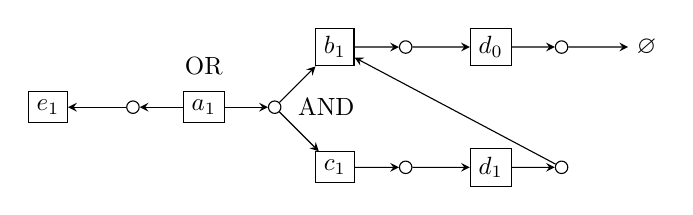
\begin{tikzpicture}[aS,scale=0.9, every node/.style={scale=0.9}]  
  	
  	\startl{a_1};
    \node[Asol,left of=a_1] (a_1s1){};
    \node[Aproc,left of=a_1s1] (e_1){$e_1$};
    \node[right = 0.1cm of a_1s] {AND};
    \node[above = 0.1cm of a_1] {OR};
    \path 
    (a_1s1) edge (e_1)
    (a_1) edge (a_1s1)
    ; 
  	\specl{above}{a_1}{b_1};
  	\link{b_1}{d_0};
  	\edl{d_0};
  	\specl{below}{a_1}{c_1};
	\link{c_1}{d_1};
    \path (d_1s) edge (b_1);
    \end{tikzpicture}

\caption{This SLCG shows the local causality of $a_1$ of the ABAN in Fig.~\ref{fig:1}, with the squares representing local states and small circles representing solution nodes}
\label{fig:2}
\end{figure}

The algorithm of SLCG construction is in Appendix~\ref{appendix:algo}.

\subsection{Limitation of SLCG}\label{limitation}
Although SLCG allows one to compute the pseudo-reachability locally without traversing the whole state space, pseudo-reachability is not equivalent to the reachability if there exist the following structures:
\begin{enumerate}[label={(\arabic*)}]
\item Cycles in SLCG
\item Firing order constraints (short for constraints) in SLCG
\end{enumerate}
To be more formal, a cycle (1) is in the form of $a_i\to\cdots\to a_i$, i.e. to access $a_i$, one has to reach $a_i$ first. This self-involvement makes the reachability inconclusive. 
Also, if a solution node has multiple successors, it creates branches.
If there are different state nodes of the same automaton in those branches \textit{i.e.} $a_i$ and $a_{1-i}$, a constraint (2) arises. 
We cannot decide the order of reaching these state nodes, because reaching one local state $a_i$ may disable the reachability of another local state.
Sometimes there exists a trajectory which accesses these state nodes in certain order, sometimes there does not exist such.
The following examples show if we ignore those limitations, SLCG does not imply real reachability.


\begin{example}\label{example:reach}
Following \textit{Example~\ref{example:SLCG}}, in Fig.~\ref{fig:2}, although there is a constraint between $d_0$ and $d_1$, $a_1$ is reachable \textit{via} trajectory $t=\acm{d_0}{b_0}{b_1}::\acm{d_0}{b_0}{b_1}::\acm{b_1}{d_0}{d_1}::\acm{d_1}{c_0}{c_1}::\acm{b_1,c_1}{a_0}{a_1}$.
\end{example}

\begin{example}\label{example:unreach}
Let us consider the ABAN given on the left in Fig.~\ref{fig:3}, with $\mathbf{\Sigma}=\{a,b,c\}$, $\mathbf{T}=\{\acm{b_0}{a_0}{a_1},\ \acm{a_0}{b_0}{b_1},\ \acm{\{a_1,b_1\}}{c_0}{c_1}\}$, the target state $\omega=a_1$. 
Both $a_1$ and $b_1$ are reachable, but they cannot be reached simultaneously.
In the SLCG, there are two branches $a_1\to b_0$ and $b_1\to a_0$.
Automata $a$ and $b$ are involved in both branches, reaching $a_1$ disables the reachability of $b_1$, \textit{vice versa}.
\end{example}

\begin{figure}[ht]
\centering
\begin{minipage}{0.4\textwidth}
\centering
\begin{tikzpicture}[apdotsimple/.style={apdot},scale=0.9, every node/.style={scale=0.9}]
\scriptsize
\TSort{(0,0)}{a}{2}{l}
\TSort{(2,0)}{b}{2}{l}
\TSort{(4,0)}{c}{2}{l}

% with delays
\path[local transitions]

	(c_0) edge node[auto] {\{$a_1, b_1$\}} (c_1)
	(a_0) edge node[auto] {\{$b_0$\}} (a_1)
	(b_0) edge node[auto] {\{$\mathbf{a_0}$\}} (b_1)
;
\TState{a_0, b_0, c_0}
\end{tikzpicture}
\end{minipage}\hfill
\begin{minipage}{0.6\textwidth}
\centering
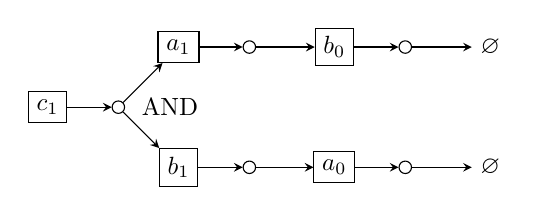
\begin{tikzpicture}[aS,every node/.style={scale=0.9}]  
  	\startl{c_1};
  	\specl{above}{c_1}{a_1};
  	\link{a_1}{b_0};
  	\edl{b_0};
  	\specl{below}{c_1}{b_1};
	\link{b_1}{a_0};
  	\edl{a_0};
  	\node[right = 0.1cm of c_1s] {AND};
\end{tikzpicture}
\end{minipage}
\caption{The ABAN and the SLCG of \textit{Example~\ref{example:unreach}}, $\alpha=\init{ a_0,b_0,c_0}$}
\label{fig:3}
\end{figure}
In \textit{Example~\ref{example:reach}}, $a_1$ is reachable, while in \textit{Example~\ref{example:unreach}}, $c_1$ is unreachable. This inconclusiveness shows the limitation of SLCG as $reach'(\alpha,\omega)$ is not equivalent to $reach(\alpha,\omega)$.
Also, as there are usually cycles in SLCG generated by feedback loops in biological regulatory networks, the existing approach does not lead to a general solution.
In the rest of this paper, we are going to discuss how to improve the performance of existing approaches and our new methods. 

\section{Heuristics for general cases}\label{sect:4}
SLCG loses its conclusiveness if there are cycles and/or constraints.
However traversing all trajectories from the initial state is computationally difficult. 
We preprocess the SLCG by removing the cycles and \textbf{OR gates}.
then perform a partial enumeration to deal with the \textbf{AND gates} which may contain constraints in the topology of SLCG.
In biological background, we can assume every component (automaton) interacts only with a small part of the whole network~\cite{akutsu2007control}.
This assumption suggests the maximum number of successors of \textbf{AND gates} in SLCG is bounded to $O(1)$, which provides the feasibility of the partial enumeration.
%Thus we can obtain a more general solution than pure static analysis (pseudo-reachability) of the reachability problem.



\subsection{Overall Process}\label{sectOverall}
Our algorithm PermReach first constructs the SLCG and filters it with pseudo-reachability. 
If pseudo-reachability does not return \textbf{False}, we then try to remove the cycles using Theorem~\ref{th:break_cycle} (introduced later).
If this removal does not work for all cycles, we launch the random choice at each \textbf{OR gate} to assign a successor solution node to be used.
In an SLCG without \textbf{OR gate}, Theorem~\ref{th:break_cycle2} (introduced later) removes all cycles.
We obtain an SLCG with \textbf{AND gates}, which can be solved by the search in permutations.
If this search fails to prove reachability, we restart the random choice.
The process loops at most $k$ times.
The value of $k$ is discussed in the benchmarks.
Detailed pseudocode is in Appendix~\ref{appendix:algo}.
\begin{itemize}
    \item Input: an ABAN $AB$, a global initial state $\alpha$, a target local state $\omega$ and a max number of iterations $k$
    \item Output: reachability $reach(\alpha, \omega)$
\end{itemize}
\begin{enumerate}
\item Construct the SLCG
\item Compute the pseudo-reachability, if $reach'(\alpha,\omega)=\mathbf{False}$, return $\mathbf{False}$
\item Detect the cycles in the SLCG and try to remove them 
\item Loop at most $k$ times:
\begin{enumerate}
    \item Launch the heuristic to remove \textbf{OR gates} 
    \item If there remain cycles:
    \begin{itemize}
        \item Back to step (4)
    \end{itemize}
    \item Tackle the SLCG with only \textbf{AND gates}, if we find a trajectory from $\alpha$ to $\omega$, return \textbf{True}; if not, back to step (4)
\end{enumerate}
\item Return \textbf{Inconclusive} (probably unreachable)
\end{enumerate}

In the following sections, we introduce the details of each step.

\subsection{Preprocessing of SLCG}\label{sectprecond}
After constructing the SLCG and filtering by pseudo-reachability, we need to deal with some structures weakening conclusiveness: cycles and \textbf{OR gates}.
\subsubsection{Detection of cycles.}
The notion of cycle can be extended to Strongly Connected Components (SCC) of size greater than 1 as an SCC may contain several nested cycles. 
Tarjan's algorithm determines the SCCs in $O(|V|+|E|)$ time~\cite{tarjan1972}. 
%As SLCG is in fact a sparse graph (the out-degree is limited to $O(1)$), the search of SCCs can be done in $O(|V|)$, \textit{i.e.} linear time.

\subsubsection{Removing cycles.}
\begin{theorem}\label{th:break_cycle}
Given a cycle $x\to \circ \to \cdots \to \circ \to x$ in an SLCG, if there is at most one incoming edge to the cycle, this cycle can be removed.
\end{theorem}
\begin{proof}
If there is no incoming edge, the target state $y$ must be in the cycle. 
The edge $y.pred\to\circ\to y$ can be removed, because the reachability of $y.pred$ requires $y$, but $y$ is the target state, which is never reached before the other local states in the SLCG are reached.
Thus the transition corresponding to this edge is never fired and the edge can be removed.
Similarly, if there is an outside incoming edge $a\to \circ \to x$, $a$ must be the successor of target state $y$, $x.pred\to\circ\to x$ is also removable.
\qed
\end{proof}


\begin{example}
    \begin{figure}[H]
        \centering
        \begin{tikzpicture}[scale=0.7]
\scriptsize
\def \n {6}
\def \radius {1.7cm}
\def \margin {8} % margin in angles, depends on the radius



\node[draw] at ({360/\n * 2}:\radius) (x) {$x$};
\node[draw, circle, minimum size=4pt, inner sep = 0] at ({360/\n * 3}:\radius) {};
\node[draw] at ({360/\n * 4}:\radius) (y) {$y$};
\node[draw, circle, minimum size=4pt, inner sep = 0] at ({360/\n * 5}:\radius) {};
\node[draw] at ({360/\n * 6}:\radius) (z) {$z$};
\node[draw, circle, minimum size=4pt, inner sep = 0] at ({360/\n * 1}:\radius) {};
\foreach \s in {3,...,\n}
{
  
  \draw[->, >=latex] ({360/\n * (\s - 1)+\margin}:\radius) 
    arc ({360/\n * (\s - 1)+\margin}:{360/\n * (\s)-\margin}:\radius);
}
\foreach \s in {1,2}
{
  
  \draw[->,dashed, >=latex] ({360/\n * (\s - 1)+\margin}:\radius) 
    arc ({360/\n * (\s - 1)+\margin}:{360/\n * (\s)-\margin}:\radius);
}
\node[left = 1.3cm of x, draw, circle, minimum size=4pt, inner sep = 0] (sol) {};
\node[left = 1.3cm of sol, draw] (origin) {$a$};
\draw[->, >=latex] (origin) to [bend left] (sol);
\draw[->, >=latex] (sol) to [bend left] (x);

\node[right = 1.3cm of z, draw, circle, minimum size=4pt, inner sep = 0] (solz) {};
\node[right = 1.3cm of solz, draw] (ext) {$w$};
\node[right = 1.3cm of ext] (etc) {$\cdots$};
\draw[->, >=latex] (z) to [bend left] (solz);
\draw[->, >=latex] (solz) to [bend left] (ext);
\draw[->, >=latex] (ext) to [bend left] (etc);
\node[above right = 0.1cm and -0.2cm of z] {OR};
\end{tikzpicture}
        \caption{SLCG containing cycle $x\to \circ \to y \to \circ \to z\to \circ \to x$}
        \label{cycle1}
    \end{figure}
    
    In Fig.~\ref{cycle1}, the pseudo-reachability of $a$ is 
    \begin{align*}
        reach'(\alpha,a)&=reach'(\alpha,x)=reach'(\alpha,y)=reach'(\alpha,z)\\
        &=reach'(\alpha,x)\lor reach'(\alpha,w)
    \end{align*}
    
    To reach $x$, we need to reach $z$, but $z$ cannot depend on $x$ as $x$ is already to be reached. 
    Self-dependence appears: $x$ is reachable if $x$ is reachable.
    Thus edge $z\to \circ \to x$ is deleted (dashed line).
\end{example}

\begin{theorem}\label{th:break_cycle2}
Given a cycle, if it contains no \textbf{OR gate}% towards outside of cycle
, all the local states in the cycles are unreachable.
\end{theorem}

\begin{proof}
Suppose an arbitrary cycle $C=a_i\to \cdots b_j\to\cdots \to a_i$, with $\to$ an edge in the SLCG.
$reach'(\alpha,a_i)\implies reach'(\alpha,b_j)\implies reach'(\alpha,b_j.next)\implies \cdots\implies reach'(\alpha,a_i)$.
According to the definition of $reach'$, $reach'(\alpha,a)=\mathbf{True}$ only if $\exists c_k\in C$ and $c_k\in \alpha$.
If there exists such $c_k$, $C$ should not exist as the reasoning stops at $c_k$ and does not form a cycle, contradiction.
$reach'(\alpha,a_i)=reach'(\alpha,b_j)=\cdots =\mathbf{False}$.\qed
\end{proof}

\subsubsection{Heuristic on OR gates.}\label{sec:OR}
For every \textbf{OR gate}, its corresponding local state is reached via only one solution node.
%we have to choose one of its successor solution nodes to access the state. 
The set of \textbf{OR gate} choices is called an \textit{assignment}.
As every \textbf{OR gate} has multiple choices, traversing all the possibilities may lead to combinatorial explosion.
We use a simple heuristic: 
choose randomly one assignment for each trial (4a) in the overall algorithm.
Then we obtain a new SLCG without \textbf{OR gate}, every state node has exactly one successor solution node.
In fact, if the target state is reachable, it is possible that exact solution is found during the trials because there are more than one path connecting $\alpha$ and $\omega$.
With Theorem~\ref{th:break_cycle} and Theorem~\ref{th:break_cycle2}, we can remove cycles and \textbf{OR gates} completely in one step.

\subsection{AND Gates in SLCG}\label{sectAndGates}
After preprocessing, we can get rid of cycles and \textbf{OR gates}.
The next step is to analyze an SLCG with only \textbf{AND gates}.
We need to find a trajectory reaching all the components of the given \textbf{AND gates} simultaneously.
These components form a joint state, and if the joint state is reachable, the corresponding transition of \textbf{AND gate} can be fired. 

In Fig.~\ref{fig:1}, $s=\{ b_1,c_1\}$ is a joint state, when $s$ is reached, transition \ac{b_1,c_1}{a_0}{a_1} is firable.
The reachability of a joint state can be then formulated as sequential reachability:
\begin{definition}[Sequential reachability]
Let $s=\{ls_1,\ldots,ls_n\}$ be a joint state, $p_1,\ldots ,p_n$ be a permutation of $1,\ldots ,n$ and $seq=ls_{p_1}::\ldots::ls_{p_n}$ be a sequence.
The sequential reachability of $seq$ is denoted %$reach(\alpha,seq)=reach(\alpha,ls_{p_1})::\ldots::reach(\alpha,ls_{p_n})$.
$REACH(\alpha,seq)=reach(s_{p_1},ls_{p_1})::\ldots::reach(s_{p_n},ls_{p_n})$, where $s_{p_1}=\alpha$, $s_{p_i}=s_{p_i-1}\cdot t_{p_i-1}$, $t_{p_i-1}$ is the obtained trajectory by the SLCG.
From initial state $\alpha$, $REACH(\alpha,seq)=\mathbf{True}$ if $s$ is reached in the order $seq$.
\end{definition}

\begin{example}\label{example:order}
Fig.~\ref{fig:5} shows the SLCG for reachability of $c_1$ in ABAN with transitions $\mathbf{T}=\{\acm{a_1,b_1}{c_0}{c_1},\acm{b_0}{a_0}{a_1},\acm{c_0}{b_0}{b_1}\}$.
$a_1$ and $b_1$ are reachable respectively but is not necessarily for the joint state $s=\{a_1,b_1\}$.
If we begin with the branch with $a_1$, $s$ is reachable with trajectory $\acm{b_0}{a_0}{a_1}::\acm{c_0}{b_0}{b_1}::\acm{a_1,b_1}{c_0}{c_1}$. 
However if we begin with the branch $b_1$, after firing $\acm{c_0}{b_0}{b_1}$, $b_0$ is no longer reachable, resulting the unreachability of $a_1$.
We have $REACH(\alpha,a_1::b_1::c_1)=\mathbf{True}$ and $REACH(\alpha,b_1::a_1::c_1)=\mathbf{False}$.
\end{example}
\begin{figure}[ht]
\centering
\begin{minipage}{0.43\textwidth}
\centering
\begin{tikzpicture}[apdotsimple/.style={apdot},scale=0.9, every node/.style={scale=0.9}]
\scriptsize
\TSort{(0,0)}{a}{2}{l}
\TSort{(2,0)}{b}{2}{l}
\TSort{(4,0)}{c}{2}{l}

% with delays
\path[local transitions]

	(c_0) edge node[auto] {\{$a_1, b_1$\}} (c_1)
	(a_0) edge node[auto] {\{$b_0$\}} (a_1)
	(b_0) edge node[auto] {\{$\mathbf{c_0}$\}} (b_1)
;
\TState{a_0, b_0, c_0}
\end{tikzpicture}
\end{minipage}\hfill
\begin{minipage}{0.57\textwidth}
\centering
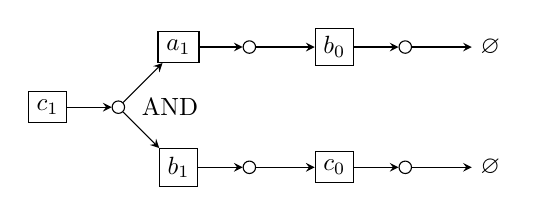
\begin{tikzpicture}[aS,every node/.style={scale=0.9}]  
  	
  	\startl{c_1};
  	\specl{above}{c_1}{a_1};
  	\link{a_1}{b_0};
  	\edl{b_0};
  	\specl{below}{c_1}{b_1};
	\link{b_1}{c_0};
  	\edl{c_0};
  	\node[right = 0.1cm of c_1s] {AND};
    \end{tikzpicture}

\end{minipage}

\caption{The ABAN and the SLCG of \textit{Example~\ref{example:order}}, $\alpha=\init{ a_0,b_0,c_0}$. 
The only difference with \textit{Example~\ref{example:unreach}} is the transition \ac{c_0}{b_0}{b_1}.
%The reachability depends on firing order of transitions
}
\label{fig:5}
\end{figure}



As the firing orders matter, we come to verify all the possible sequential reachabilities of certain joint state to verify its reachability.

\begin{proposition}\label{theoperm}
Given joint state $s=\{ls_1,\ldots,ls_n\}$, with all the local states in $s$ are reachable: $reach(\alpha,ls_i)=\mathbf{True},\ \forall i\in[1,n]$, the set of permutations of $s$ is denoted $Perm(s)=\{(ls_1::ls_2,::\ldots ::ls_n),\ \cdots,\ (ls_n::ls_{n-1}::\ldots,::ls_1)\}$. $\bigvee_{i\in Perm(s)} REACH(\alpha,i)=\mathbf{True}$ is a sufficient condition of $REACH(\alpha,s)=\mathbf{True}$.
\end{proposition}
\begin{proof}
If $\exists perm_i\in Perm(s)$ s.t. $REACH(\alpha,perm_i)=\mathbf{True}$, $s$ can be reached according to the order in $perm_i$.
To reach $s$, every local state in SLCG is mandatory to be reached, as according to the definition of SLCG, it is the smallest structure which contains all the needed local states and transitions for the target state. As long as there is no \textbf{OR gates}, all the transitions in the SLCG must be fired to reach the target state.
For solvable constraints, $Perm(s)$ can cover some of the admissible orders.
\qed\end{proof}

In case where the successors of certain \textbf{AND gate} contain other \textbf{AND gates}, we cannot directly obtain its reachability because the reachability of the successor \textbf{AND gates} are unknown.
We analyze first the simple \textbf{AND gates} $simp$, i.e. the successors of $simp$ do not contain any \textbf{AND gates}.
If all local states within $simp$ are reachable via the search of permutations, we can update the initial state by firing all the transitions and also update the SLCG by deleting the successors of $simp$. 
Then we restart this process from new simple \textbf{AND gates} until we reach finally the target state.

However the method of PermReach is not complete. 
If there are constraints in different branches, traversing all the permutations may be not sufficient to find admissible trajectories towards the target state.
In Fig.~\ref{FigConflictInForks}, among the simple \textbf{AND gates}, if $sol_{c_1}$ is solved first, automaton $d$ will be at the state $d_1$, which disables the reachability of $b_1$.
The trajectory towards $a_1$ may not be retrievable by PermReach even if $a_1$ is reachable.
\begin{figure}[ht]
\centering
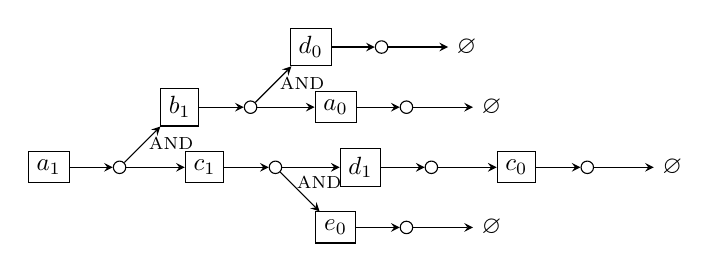
\begin{tikzpicture}[aS, every node/.style={scale=0.9}]  
  	
	\startl{a_1};
	\specl{above}{a_1}{b_1};
	\specl{above}{b_1}{d_0};
	\edl{d_0};
	\link{b_1}{a_0};
 	\edl{a_0};
	\link{a_1}{c_1};
 	\link{c_1}{d_1};
 	\link{d_1}{c_0};
 	\edl{c_0};
 	\specl{below}{c_1}{e_0};
 	\edl{e_0};
 	\node[above right = 0.05cm and 0.2cm of a_1s] {\scriptsize AND};
 	\node[above right = 0.05cm and 0.2cm of b_1s] {\scriptsize AND};
 	\node[below right = -0.05cm and 0.1cm of c_1s] {\scriptsize AND};
    \end{tikzpicture}
\caption{Counterexample of PermReach, $\alpha=\init{ a_0,b_0,c_0,d_0,e_0}$. 
$reach(\alpha,a_1)$=\textbf{True} but \textbf{Inconclusive} is given by PermReach.
}\label{FigConflictInForks}
\end{figure}
%The statement above is the worst case: in reality, all \textbf{AND gates} are not necessarily composed of exact $I$ components, and permutations are determined to be unreachable before verification as its subsets may have been confirmed unreachable in other tentatives.

%For example: given an \textbf{AND gate} $sol_a=b\land c\land d$, where $b,c,d$ are local states.
%Normally 6 realizing orders need checking: $b::c::d$, $b::d::c$, $c::b::d$, $c::d::b$, $d::b::c$ and $d::c::b$. 
%If we find the order $b::c$ is not realizable when verifying the first realizing order, then we do not have to verify the reachability of $b::c::d$ and $b::d::c$ where $b$ occurs before $c$. $d::b::c$ is not included, because firing $d$ changes its state before firing $b::c$.

\section{Implementation and benchmarks}\label{sect:5}
The overall process in section~\ref{sectOverall} is implemented in Python\footnote{Implementation and testing data sets are available at \url{https://github.com/XinweiChai/LCG-in-ASP}}. 
To validate our approach in large \textit{in silico} networks of biological systems, we take T-cell Receptor model (TCR)~\cite{saez2007logical} and epidermal growth factor receptor model (EGFR)~\cite{samaga2009logic} as examples, with the former one containing 95 components and 206 transitions and the latter one containing 104 components and 389 transitions respectively. 

These models are originally Boolean networks.
According to Appendix~\ref{appendix:trans}, they can be translated to ABANs. We then take several automata as input, varying exhaustively their initial states combinations ($2^{init\_state}$), take the reachability of the states of another automata set as output.
We first test the performance of traditional model checkers, Mole\footnote{\url{http://www.lsv.fr/~schwoon/tools/mole}} and NuSMV\footnote{\url{http://nusmv.fbk.eu}}, in which Mole turns out to be timeout for 6 in 12 outputs, and all timeouts for NuSMV in model EGFR.
Due to the big state space, traditional model checkers are not applicable. 

To validate our approach, we first use a small model: $\lambda$-phage model~\cite{thieffry1995dynamical} to compare with an alternative static reachability analyzer Pint~\cite{pauleve2012}. In this model with 4 components and 12 transitions, our result shows full conclusiveness while Pint returns the reachability of $[cll_1=1]$ with inconclusive.
Big networks TCR and EGFR are already tested by Folschette \textit{et al.} modeling in Asynchronous Automata Network with priority~\cite{folschette2015}. 
In the TCR tests, PermReach gives exactly the same result as~\cite{folschette2015} did as there is no inconclusive cases. As for EGFR tests, PermReach shows also full conclusiveness while Asynchronous Automata Network with priority does not.
%in his paper, there are about Almost all the examples in this paper are ``inconclusive'' in Pint, but they are solvable \textit{via} the presented heuristic technique. In~\cite{folschette2015}, Folschette \textit{et al.} ran tests over the possible variations of 13 input nodes (different initial states), and observed the reachability of other 12 components. In total $12\times 2^{13}=98,304$ instances are tested. Among these tests, there are 9,986 (10,16\%) inconclusive instances. We conducted tests on these instances and found out they are conclusive in our methods.

\begin{table}[ht]
\centering
    \begin{tabular}{|c|c|c|c|c|c|c|}
    \hline
  	Model	&\multicolumn{2}{c|}{$\lambda$-phage}	&	  \multicolumn{2}{c|}{TCR} & \multicolumn{2}{c|}{EGFR}  \\
    \hline
    Inputs&\multicolumn{2}{c|}{4}	&	  \multicolumn{2}{c|}{3} & \multicolumn{2}{c|}{13}\\
    \hline
    Outputs&\multicolumn{2}{c|}{4} &	  \multicolumn{2}{c|}{5} & \multicolumn{2}{c|}{12} \\
    \hline
    Total tests&\multicolumn{2}{c|}{$2^4\times 4=64$} & \multicolumn{2}{c|}{$2^3\times 5=40$} & \multicolumn{2}{c|}{$2^{13}\times 12=98,304$}\\
    \hline
    Analyzer  &  Pint       &\textbf{PermReach}    &  Pint       &\textbf{PermReach}   &  Pint       &\textbf{PermReach}             \\
    \hline
    Reachable    & 36(56\%)& 38(59\%)   &  \multicolumn{2}{c|}{16(40\%)}  & 64,282(65.4\%)&74,268(75.5\%)\\
    \hline
    \textbf{Inconclusive} & \textcolor{red}{\textbf{2(3\%)}}&\textcolor{blue}{\textbf{0(0\%)}}& \multicolumn{2}{c|}{0(0\%)}    &\textcolor{red}{\textbf{9,986(10.1\%)}}&\textcolor{blue}{\textbf{0(0\%)}}  \\
    \hline
    Unreachable     &  \multicolumn{2}{c|}{26(41\%)} &  \multicolumn{2}{c|}{24(60\%)} &24,036(24.5\%)&24,036(24.5\%)\\
    \hline
    Total runtime &  $<1$s       &  $<1$s &  \textbf{7s}       &  \textbf{0.85s}        & \textbf{9h50min}              & \textbf{15min31s}      \\
    \hline
    \end{tabular}
\caption{Results of the tests on large-scale examples using Intel Core i7-3770 CPU, \@3.4GHz, 8.00G RAM. 
Column “Pint” gives the related results on ANs, while column “PermReach” gives the results for ABANs. 
“True”, “Inconclusive” and “False” give respectively the number of different results of reachability, while “Max time” and “Total time” depict respectively the maximum time of the individual computations.}
\label{tab:2}
\end{table}

Besides the tests done by others, we also carry tests on some randomly generated ABANs to check the generality and the time-performance of PermReach. 
Given the number of transitions, for every transition $tr$, the head $a_h$ is randomly chosen from $\mathbf{LS}$, the first element of the body $A_1$ is chosen from $\mathbf{LS}_1=\mathbf{LS}\setminus \{a_h,a_{1-h}\}$.
For $i>1$, if $A_{i-1}=b_x$ exists, we generate $A_i$ with an 80\% probability, choosing from $\mathbf{LS}_i=\mathbf{LS}_{i-1}\setminus \{b_x,b_{1-x}\}$. 
 
One test is on the different numbers of automata with the same density (average number of transitions per automaton) of ABAN. Fixing the density to 3, we vary the number of automata from $10,20,\ldots,100,200,\ldots,1000$.
In the instances with less than 300 automata, the runtime of each reachability check is less than 0.1s.
Fig.~\ref{fig:sizeTest} shows the average runtime is less than 5 seconds even if there are 1000 automata. 
Moreover, the longest runtime among the test sets is less than 20s. 
Because we stop the computation if one reachability check takes more than 20s and we note it as timeout.
We find no timeout case.
\begin{figure}[ht]
    \subfigure[0.5\textwidth][ABAN density fixed to 3]{
    %\begin{tikzpicture}[>=stealth,scale=0.6,line width=0.8pt]
%\scriptsize
%% % % % % % % % % % % % % % %
% 
%\pgfmathsetmacro{\ticker}{0.125} 
% 
%\coordinate [label=225:0](A) at (0,0);
%\coordinate (B) at (0,5);
%\coordinate (C) at (7.5,5);
%\coordinate (D) at (7.5,0);
%\draw(A)--(B)--(C)--(D)--cycle;
% 
%\coordinate [label=left:{\scriptsize runtime(s)}](E) at ($(B)+(1,0.2)$);
%\coordinate [label=below:{\scriptsize components}](F) at ($(D)+(0,-0.3)$);
% 
%\foreach \i/\texti in {100,300,...,1000} {
%\draw (0.01*\i*0.7,0) --(0.01*\i*0.7,\ticker) node[label=below:\texti]{};
%}
%\foreach \i in {200,400,...,1000} {
%\draw (0.01*\i*0.7,0) --(0.01*\i*0.7,\ticker);
%}
%
%\foreach \j/\textj  in {1,2,3,4} {
%\draw (0,\j) --(\ticker,\j) node[label=left:\textj]{};
%}
%
%
%\coordinate (1) at (1*0.7,0.029);
%\coordinate (2) at (2*0.7,0.079);
%\coordinate (3) at (3*0.7,0.209);
%\coordinate (4) at (4*0.7,0.330);
%\coordinate (5) at (5*0.7,0.729);
%\coordinate (6) at (6*0.7,0.948);
%\coordinate (7) at (7*0.7,1.379);
%\coordinate (8) at (8*0.7,2.102);
%\coordinate (9) at (9*0.7,3.416);
%\coordinate (10) at (10*0.7,4.58);
%\draw(1)--(2)--(3)--(4)--(5)--(6)--(7)--(8)--(9)--(10);
% 
% 
% 
%\end{tikzpicture}
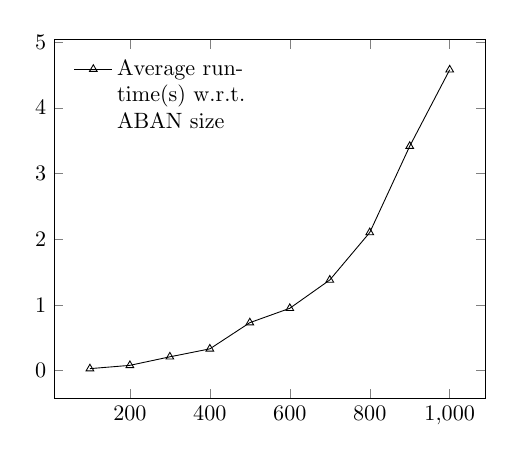
\begin{tikzpicture}[scale=0.8]
    \begin{axis}%[legend pos=north west]
       \addplot[mark=triangle] coordinates{
        (100,0.029)
        (200,0.079)
        (300,0.209)
        (400,0.330)
        (500,0.729)
        (600,0.948)
        (700,1.379)
        (800,2.102)
        (900,3.416)
        (1000,4.58)
        };
        \addlegendentry{Average runtime(s) w.r.t. ABAN size}
    \end{axis}
\end{tikzpicture}
    \label{fig:sizeTest}
    }
    \subfigure[0.5\textwidth][ABAN size fixed to 20]{
        \centering
    %\begin{tikzpicture}[scale=0.8]
%\begin{axis}[xlabel=ABAN density,ylabel=runtime (s)]
%\addplot[mark=o] coordinates {
%        (1,0.01)
%        (2,0.01)
%        (3,0.02)
%        (4,0.02)
%        (5,0.32)
%        (6,0.92)
%        (7,1.24)
%        (8,1.08)
%        (9,1.02)
%        (10,0.87)
%        (11,0.75)
%        (12,0.42)
%    };
%\addlegendentry{Average runtime(s) w.r.t. ABAN density};
%\end{axis}
%
%\end{tikzpicture}
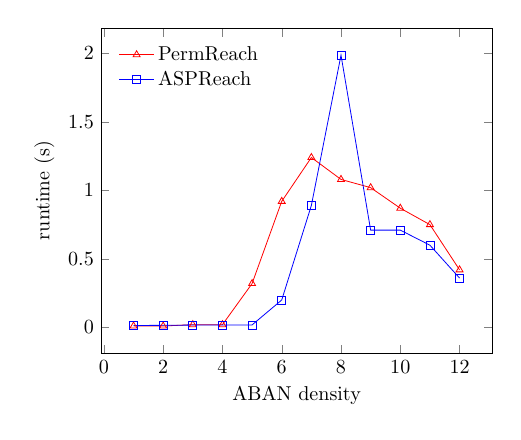
\begin{tikzpicture}[scale=0.725]
\begin{axis}[xlabel=ABAN density,ylabel=runtime (s)]
\addplot[mark=triangle,color=red] coordinates {
        (1,0.01)
        (2,0.01)
        (3,0.02)
        (4,0.02)
        (5,0.32)
        (6,0.92)
        (7,1.24)
        (8,1.08)
        (9,1.02)
        (10,0.87)
        (11,0.75)
        (12,0.42)
    };
\addlegendentry{PermReach};
       \addplot[mark=square,color=blue] coordinates{
        (1,0.014)
        (2,0.015)
        (3,0.017)
        (4,0.017)
        (5,0.018)
        (6,0.2)
        (7,0.89)
        (8,1.987)
        (9,0.710)
        (10,0.71)
        (11,0.6)
        (12,0.36)    
        };
        \addlegendentry{ASPReach}
\end{axis}
\end{tikzpicture}
    \label{fig:inconcTest}
    }
    \caption{Runtime of PermReach on random ABANs}
\end{figure}
Another test is on the different density with the same number of automata. 
Fixing the number of automata to 20, we vary the density of the transitions from 1 to 12.
We find the runtime peak is at density 7, a possible explanation is that even the topology of the network is more complex with the growth of the density, more transitions lead to more paths from the initial state to the target state, thus PermReach succeeds with less trials.
Among the reachability results, the ABANs of high density have more \textbf{True}s than those of low density.
Last but not least, in the implementation, we set arbitrarily iteration limit $k=100\times|\mathbf{OR\  gates}|+1$. 
Apart from handmade counterexample in Fig.~\ref{FigConflictInForks}, there is no case in the tests where the iterations reach $k$ times.
%In the configuration of the heuristic approach, if there are less than 20 \textbf{OR gates} after preprocessing in Section~\ref{sectprecond}, the computation will be shifted from heuristic to global search as the size of enumeration is acceptable.
%There are only 11 \textbf{OR gates} in EGFR model, therefore the results are firmly conclusive. 


To sum up, PermReach has a better time performance than traditional model checkers based on global search (Mole and NuSMV); furthermore, it is more conclusive and has a better time performance than abstract analyzer (Pint).

\section{Conclusion and future work}\label{sect:6}
This paper proposes an expressive formalism ABAN to study the reachability problem. 
Due to the complexity of global search and inconclusiveness of pure static search, developing a heuristic technique based on static analysis becomes a feasible choice.
The heuristic method PermReach reproduces the system dynamics by searching admissible orders of transitions.
The benchmarks display its conclusiveness and efficiency.

The computation of permutations could however be heavy in the networks bigger than the tests in this paper and is still not fully conclusive. 
To speed up the whole procedure and improve the conclusiveness, we thus plan to apply SAT (Satisfiability) solvers or Answer Set Programming (ASP) to refine the analysis of transition orders. 
In addition, we may consider an extension of PermReach to multivalued models.


\bibliographystyle{plain}
\bibliography{bib.bib}   % name your BibTeX data base
\appendix
\section{Transformation from general BNs to ABANs}\label{appendix:trans}

Given Boolean functions $v_i(t+1)=f_i(\mathbf{V}_i)$, with $\mathbf{V}_i$ the set of participating variables among $v_1(t),\cdots,v_n(t)$.
Boolean functions could be transformed to equivalent CNF (conjunctive normal form) and DNF (disjunctive normal form) if the length of Boolean functions is limited to $O(1)$~\cite{miltersen2005converting} which is often the case.
\begin{proposition}[Transformation from BN to ABAN]
Given a BN $G_B=(V,F)$, with its functions in CNF form $v^i(t+1)=A_1\land\ldots A_j \ldots\land A_n$ and DNF form $v^i(t+1)=A'_1\lor\ldots A_k\ldots\lor A'_m$, an equivalent ABAN $AB$ has transitions $A_j\to v^i_1$ and $\lnot A_k\to v^i_0$ where $A_j$ are disjunctions and $A'_K$ are conjunctions.
\end{proposition}
\begin{example}
Let $G_B=(V,F)$ a BN with $V=\{a,b,c,d,e\}$, and has only one Boolean function, $F=\{f(a)= (b\lor c)\land(d\lor e)\}$, we have 
$f(a)=(b\land d)\lor(b\land e)\lor(c\land d)\lor(c\land e)$, and $\lnot f(a)=(\lnot b\land \lnot c)\lor(\lnot d\land \lnot e)$. 
The equivalent ABAN is then constructed: 5 automata $\mathbf{\Sigma}=\{a,b,c,d,e\}$, with transitions: $\mathbf{T}=\{\acm{b_1,d_1}{a_0}{a_1},\ \acm{b_1,e_1}{a_0}{a_1},\ \acm{c_1,d_1}{a_0}{a_1},\ \acm{c_1,e_1}{a_0}{a_1},\ \acm{b_0,c_0}{a_1}{a_0},\ \acm{d_0,e_0}{a_1}{a_0}\}$.
\end{example}

\section{Algorithms}\label{appendix:algo}
%The construction of an SLCG is realized by iterative updates:

\begin{algorithm}[ht]
\begin{algorithmic}
\State Input: an ABAN $AB=(\mathbf{\Sigma},\mathbf{L},\mathbf{T})$, an initial state $\alpha$, a target state $\omega$
\State Output: SLCG $l=(V_\st,V_\sol, E)$
\State Initialization: 
$Ls\gets \{\omega\}$, $V_\st\gets\varnothing$, $V_\sol\gets \varnothing$, $E\gets \varnothing$
\While{$Ls\neq \varnothing$}
    \State $Ls=Ls\backslash V_\st$
	\For{$a_i\in Ls$}
		\State $Ls\gets Ls\backslash \{a_i\}$
		\If{$a_i\in \alpha$}
			%\State $a_i{\rm .next}=sol_{a_i}$
			%\State $V_\sol\gets V_\sol\cup \{(a_i,\varnothing)\} $
			\State $E\gets E\cup \{(a_i,\varnothing)\} $
            %\State $sol_{a_i}{\rm .next}=\varnothing$
    	\Else
    	    \State{\textcolor{gray}{// Choose the transitions reaching $a_i$, i.e. with body $a_{1-i}$}}
    		\For{$sol=A\to a_{1-i}\in \mathbf{T}$}
    		    \State $V_\sol\gets V_\sol\cup \{sol\}$
    		    \State $E\gets E\cup \{(a_i,sol)\} $
    			%\State $a_i{\rm .next}\gets a_i{\rm .next}\cup sol$
    			\State $V_\st\gets V_\st\cup {A}$
    			\For{$b_j\in A$}
    				%\State $sol{\rm .next}\gets b_j$
    				\State $E\gets E\cup \{(sol,b_j)\} $
    			\EndFor
    			\State $Ls\gets Ls\cup A$
                \State $V_\st\gets V_\st\cup Ls$
    		\EndFor
    		\State$V_\sol\gets V_\sol\cup a_i{\rm .next}$           
    	\EndIf
	\EndFor
\EndWhile
\State\Return{$(V_\st,V_\sol,E)$}
\end{algorithmic}
\caption{Construction of SLCG}\label{AlgConstructLCG}
\end{algorithm}

\begin{algorithm}[ht]
\begin{algorithmic}
\State Input: an SLCG $l=(V_\st, {V_\mathrm{solution}},E)$, an initial state $\alpha$, a target state $\omega$
\State Output: a Boolean $reach'$
\Procedure{pseudoReach}{$s$}
\State \textcolor{gray}{// If $\omega$ is in initial state, it is already reached}
\If {$\omega\in \alpha$}
   \Return \textbf{True}
\EndIf
%\State \textcolor{gray}{// If no solution nodes leads to $s$, $s$ is unreachable}
\State \textcolor{gray}{// The reachability of $s$ depends on its successor solution nodes}
\If {$\not\exists (s,sol) \in E$}
    \Return \textbf{False}
\EndIf
\For{each $(s,sol) \in E$}
    \If{\Call{fireable}{$sol$}}
    \Return \textbf{True}
    \EndIf
\EndFor
 \Return \textbf{False}
\EndProcedure
\Procedure{fireable}{$sol$}
\For{each $(sol,s') \in E$}
    \If{\Call{pseudoReach}{$s'$}}
    \Return \textbf{False}
    \EndIf
\EndFor
\Return \textbf{True}
\EndProcedure
\end{algorithmic}
\caption{Pseudo-reachability $reach'$}\label{algPseudo}
\end{algorithm}

\begin{algorithm}[ht]
\begin{algorithmic}
\State Input: an SLCG $l=(V_\st,V_\sol, E)$, initial state $\alpha$, target state $\omega$, an integer $k$
\State Output: reachability $r$
\State \textcolor{gray}{// 1) Try to break cycles}\label{delete_cycle_begin}
\For{each $ scc=(V'_{\mathrm{state}},V'_{\mathrm{solution}}) \in \mathrm{SCC}(l)$ with $V'_{\mathrm{state}} \subseteq V_\st,V'_{\mathrm{solution}}\subseteq V_\sol$}
    \If{$scc$ has less than one incoming edge}
        \For{each $v \in V'_{\mathrm{state}}$}
            \If {$\exists(v,v')\in E, v' \in (V_\sol \setminus V'_{\mathrm{solution}})$}
                \State $E\gets E\backslash \{(v,v'')|v''\in V'_{\mathrm{solution}},(v,v'')\in E\}$
            \EndIf
        \EndFor
    \EndIf
\EndFor \label{delete_cycle_end}
\State{\textcolor{gray}{// 2) Remove useless nodes/edges}} \label{prune_begin}
\State pruned = true
\While{pruned}
    \State pruned = false
    \For {$v \in V_\st$}
        \If{$\not\exists(v,v')\in E$}
            \State $V_\st \gets V_\st\backslash \{v\}$; $E\gets E\backslash \{ (v'',v)\in E\}$
            \State $E\gets E\backslash \{ (v'',sol)\in E | sol \in \{sol = (A \rightarrow a) \in V_\sol | v \in A\}\}$
            \State $V_\sol \gets V_\sol\backslash \{sol = (A \rightarrow a) \in V_\sol | v \in A\}$
            \State pruned = true
        \EndIf
    \EndFor \label{prune_end}
\EndWhile
\State \textcolor{gray}{// 3) Check pseudo-reachability} \label{pseudo_reach_begin}
\If {PSEUDOREACH$(l)=\textbf{False}$}
    \State \Return $\mathbf{False}$
\EndIf \label{pseudo_reach_end}

\State \textcolor{gray}{// 4) main search loop} \label{main_loop_begin}
\For{each $i$ in $1\ldots k$}
    \State $l'=(V'_{\mathrm{state}}, V'_{\mathrm{solution}},E')\gets(V_\st, V_\sol,E)$
    \For{$v \in V'_{state}$} \textcolor{gray}{// Treat each OR gates}
        \State pick a random element $(v,v') \in E'$
        \State $E'\gets E' \backslash  \{(v,v'') \in E'| v''\neq v'\}$
    \EndFor
    \If{$l'$ contains cycles}
        \State \textbf{Continue}
    \EndIf
    %\State $(r,t)\gets\mathrm{ASPsolve}(l')$
    \State Obtain simple \textbf{AND gates} $simp$ from $l'$
    \While{$simp\neq \varnothing$}
        \State $re\gets\mathbf{False}$ \textcolor{gray}{// check the reachability of $simp$, if true, update initial state}
        \For{$i \in perm(simp)$} 
            \If{$REACH(i)=\mathbf{True}$}
                \State $re\gets\mathbf{True}$
                \State \textbf{Break}
            \EndIf
        \EndFor
        \If{$re=\textbf{True}$}
            \State update $\alpha$ by firing transitions in $simp$
            \State $V'_{\mathrm{solution}}\gets V'_{\mathrm{solution}} \backslash simp$
        \Else
            \State \textbf{Break}
        \EndIf
        \State Obtain simple \textbf{AND gates} $simp$ from $l'$
    \EndWhile
    \If{$re=\textbf{True}$}
        \Return{$\mathbf{True}$}
    \EndIf
\EndFor \label{main_loop_end}
\State \Return{$\mathbf{Inconclusive}$}
\end{algorithmic}
\caption{PermReach}\label{algOverall}
\end{algorithm}

\end{document}